\chapter{Griqualand West History}    

Griqualand West owes its origin to Adam Kok, a slave whose strong sense of duty earned him his freedom. He was intially allowed to settle on a farm near St.Helena Bay. He became the patriarchal head of state of the Grigrigua tribe as well as some Namaquas and a group known as 'Basters', the progeny of a mixture of the indigenous Hottentots and Europeans. However, in the main the group was of Hottentot descent.


\ph[width = .98\textwidth]{../cape-of-good-hope/Maps/south_africa_1885.jpg}{1885 Map of South Africa}


In the main, however, the group was of Hottentot descent. Adam Kok was recognised as the head of the 'Griquas' by the Cape Government. In about 1750 he and his followers moved to the Kamiesberg in Namaqualand. In 1795, shortly before his death, he handed over leadership to his son Cornelis.

At about the same time a the genesis of the Kok clan, a group of Basters with allegiance to Barend Barends and his brother Nicholaas, banded together. They too moved north towards the Orange River in the vicinity of the Prieska Drift.

\begin{marginfigure}
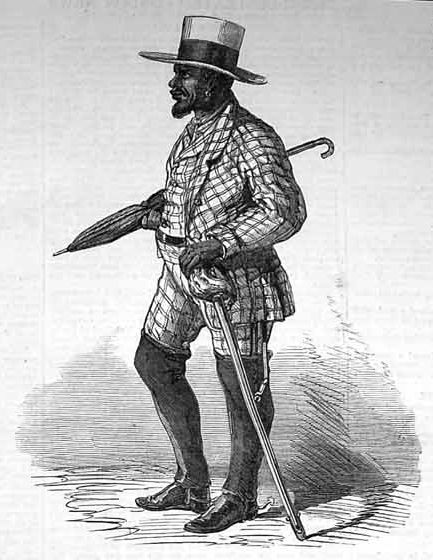
\includegraphics[width=1.0\textwidth]{../griqualand-west/adam-kok.jpg}
\caption{Captain Adam Kok, Chief of the Griquas, London Illustrated News, 1867.}
\end{marginfigure}

These people were nomadic but following a disastrous drought, they established a permanent settlement, based on agriculture, in 1803-04. This was North of the Orange River, along a series of springs in the area of Prieska to Danielskuil, where the Basters were joined by Koranna and Bechuana tribesmen.

A presence of the South African Missionary Society had meanwhile been established in 1800 for the Bechuana people at what was then known as New Lettakoo, about 320 km to the North.

The London Missionary Society established a mission station at Klaarwater, which in 1813 was named Griquatown. William Anderson was appointed the station's first superintentent. It became the capital of the settlement and the inhabitants referred to themselves collectively as Griquas. The population of Klaarwater and the surrounding district had by then grown to 1300. From1816, the New Lettakoo mission station had been administered by the London Missionary Society and a year later the mission was moved nearer to Kuruman River, about 20 km from the present town of Kuruman. The mission thence being known as Kuruman Mission. It was superintended from 1821 onwards by Robert Hamilton, who was replaced in 1824 by the famous missionary couple Robert and Mary Moffat. In that year the station was again moved to about 4 km from the present Kuruman.

Diamonds were discovered in Griqua territory in 1866 and the question of sovereignity over the area assumed politicalimportance. Claims to it were made by the Griqua paramount chief, Nicholas Waterboer, who had succeeded Adam Kok, as well as by the South African republic and the Orange Free State.

the Keate Award in October 1871 determined the issue in favour of waterboer. However, the diamond diggers along the Vaal River disputed the award and set up an independent republic. This was short lived and the territory annexed by Great Britain 10 days later.

In 1873, Griqualand west was constituted a separate British Colony, but it was annexed to the Cape Colony by an Act of Parliament on 5 August 1879 merging with it in 1880 after the Griqua rebellion of 1878 that was supressed.

Andries Waterboer, who had been an assistant teacher at the mission school, was elected chief of the Griquas in 1821 and a form of local government ensued. In 1823 the settlement numbered 4000.

(See timeline of Griqualand West History).

Postal History of Griqualand

The early postal history of Griqualand is dominated by missionary letters disptached privately. Both correspondence emanating from Hamilton or Moffat exists. These were both official as well as private letters. they bear no markings.

When John Melville was appointed as a government agent in 1822 mail was probably being sent in the officia bag. By 1824 letters were being conveyed by wagon.

In 1828, the nearest post office to Griquatown was at Graaff-Reinet, more than 400 km away. With the opening of a post office at Colesberg in 1841, Griquatown was closer to stablished postal routes, but even this office was still about 400 km distant.

It appears at this stage tranmission of letters from Griquatown to Colesberg was largely dependednt on 'favourable opportunity'. From Colesberg the letters were sent to Graaf-Reinet, and then via Cradock to Port Elizabeth. Moffat complained in March 1851 that 'opportunities between the nearest post office at Colesberg and this (Griquatown) are sometimes far few and between.

The opening of a post office in the village of Hopetown in 1855, just over 100 km from Griquatown, brought facilities considerably closer.

Postal developments after the discovery of diamonds in 1866 was rapid.The Diamond News of 15 October 1870 stated that 'Last Saturday was the first day on which the Free State post came into operation here. Postmaster Palier informs us that on that day he issued 670 letters and 705 Newspapers...'

The notification refers to the post office opened at Pniel on the south bank of the vaal River in the Orange River Sovereignity. The offices at Klip Drift on the North bank and Du Toit's pan were opened shortly afterwards. It is likely that mail was processed through the Free State until the opening of the Klip Drift office.

In September 1870 tenders were invited to convey the mail from Hopetown to Klip Drift. Untilthen the Hopetown residents had to cross the Vaal by ferry to collect their mail.

The first mailto Klipdrift was dispatched from Cape Town to the diamond fields on 14 January 1871. The mail contained 16 letters and 26 books and nespapers and was conveyed by passenger wagon. Mr. A Von Bressendorf was the postmaster.

The first mailcart from Hopetown to Klip Drift was in March 1871. In March 1872 two other post offices were opened one at De Beers New rush and the other at Du Toit'sPan.

In 1873-74 the Griqualand West Post Offices were as shown in the table below:      